% (c) 2020 Stefan Antonowicz
% Based off of tex found at https://github.com/ludus-leonis/nipajin
% This file is released under Creative Commons
% Attribution-NonCommercial-ShareAlike 4.0 International License.
% Please do not apply other licenses one-way.

\renewcommand{\yggTheBand}{%
  \mychapter{The Band}{the-band}
}

\renewcommand{\yggTheBandText}{%
  
  \mysection{The Totality of Ygg}{band-totality-ygg}

  At the center of nothing lie the immeasurable gardens of the Prime \TheAuthority; from the gardens' center grows Ygg, the tree of the Multiverse.  Beneath its infinite branches \TheAuthority dreams of existence, and when \TheAuthority awakens it will mean THE END.  Overhead, uncountable plumules grow from boundless limbs (each a universe in their own right), and Time marches steadily through the tributaries of Ygg's phloem.  The Totality refers to the gardens, \TheAuthority, the Small Gods that play silently at his bedside, and everything that exists beneath them.

  Growing inside one of these buds, at the off-center of a lenticular galaxy, a gas giant spins slowly around a star in a modest elliptical orbit; around this goliath five moons are caught in a gravitiational embrace.  The natives of these moons call the porphyry gas giant Tartarus, its star Helios - and have named themselves as well:  Acheron, Cocytus, Phlegethon, Styx, and Lethe.


\begin{center}
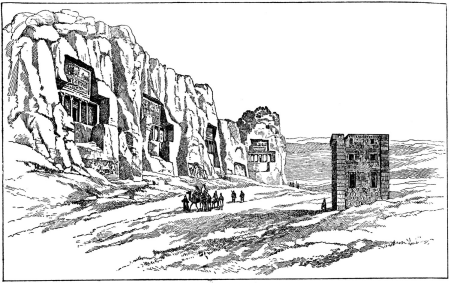
\includegraphics[scale=.5]{the_band}
\end{center}



  The moons each have a land mass about twice the size of Asia; they are roughly equidistant from one another, meaning that from any single moon you can see two other moons glittering in the night sky.  Tartarus is faintly visible in the morning light; as the day progresses, a crescent appears as Helios alights upon the visible side of the planet.  Tartarus begins waxing, its fullness heralding the coming of night.  At dusk, the light of Tatarus provides significant illumination - enough to read by - but becomes more and more shadowed as the night progresses and the two moons become more and more vibrant. It is darkest before dawn; Helios rises and hides her face behind Tartarus in a spectacular eclipse.  During this time it is pitch dark, a time of great mischief, fear, and terror until Helios peeks her face from behind Tartarus to begin the wheel anew.

  \myital{Ed: I happened to have picked Acheron for these rules, but I hope you'll feel comfortable picking something else - either around this star, or another, or in another universe entirely.  Wherever you see "Acheron" written, let your mind run wild.}

  \mysection{Acheron}{band-acheron}

  30,000 years ago, your ancestors stopped their incessant wandering and began settling down onto farms - farms which grew to cities, and civilizations.  Scores if not hundreds of empires have risen and fallen on Acheron, each successive generation (re)building on the broken bones of whatever came before.  The wreckages of the past dot Acheron - not just physically in ruined buildings and destroyed palaces, but socially, spirtually, and morally.  The infection of these crumbling societies seeps into your everyday life.  You are a cargo cult of a cargo cult stumbling in the shadow of titans.

  This makes Acheron very dangerous outside of the borders of cities.  Four major cities are the capitals of the four provinces; smaller towns and hamlets ooze like fungus here and there between forgotten crypts, feral ecosystems, abandoned cities, and rotting technology; multiple vast empires of Unseelie fight and die in the Veins of the Earth beneath the surface of the moon.  The mortals huddle together in their "civilizations", hoping the campfires keep the wolves at bay.

  But where some might despair, others find opportunity ...  


  \mysection{Making a Living}{band-making-a-living}

  This amalgam of peoples building on the bones of civilizations has lead to the creation of interesting economies.  All precious metals (silver and gold) have been mined, pressed into coins and candelabra - but re-buried and lost when their nations fell.  Similarly, iron may have once been plentiful but now exists only in tools, armor, weapons; ingots and coins.  Practically, this has made iron, silver, and gold the uniform system for measuring credits and debts for the past few millenia.

  You are an Adventurer who, for your own reasons, has decided to "rescue" this iron, silver, and gold from the tombs, caverns, and dungeons of Acheron.  It is dangerous to go alone, however - you need to be in a Band.  Adventurers in the Totality of Ygg form caravans, companies, and expedition parties to loot treasures, rob tombs, unearth eldritch horrors, and generally eke out a living.  Your Band of like-minded adventurers will work together towards the acquisition of these riches; high danger, high reward.  


  \mysection{Adventurer Creation}{band-creating-adventurer}

To create an adventurer:

\mybold{Step 1: Define your \mylink{Tangible Stats}{tangible-stats} and \mylink{Intangible Stats}{intangible-stats}}

For your Tangible Stats, choose one of the following dice combinations, and assign a single die to \VIG, \DEX, \INT, and \FOC ("bigger" dice are better)

\mybullet {
  \item  d10, d10, d6, d6
  \item  d10, d8, d8, d6
  \item  d8, d8, d8, d8
}

Your Intangible Stats start at a d6 (though these may be increased during character creation)


\mybold{Step 2: \mylink{Initial Skills}{skills}}

Write down the 7 basic \mylink{Skills}{skills}: Bushcraft, Eyeball, Listen, Lore, Math, Salt, and Travel.  You start Trained in one of these skills (d8,+1) but Untrained in the rest (d4,+0)

\mybold{Step 3: \mylink{Initial Saves}{saves}}

Write down the 3 basic \mylink{Saves}{saves}:  Hex, Toxins, and Doom.  You start Preserved in one of these Saves (d8,+1) but Defenseless in the other 2 (d4,+0)

\mybold{Step 4: \mylink{Initial \DEATH}{combat-dying}}

You start with a Precarious (d3) \DEATH.


\mybold{Step 5: Mortal or Unseelie?}

Decide if your adventurer is \mylink{Mortal}{mortals} or \mylink{Unseelie}{unseelie}.  If you're Mortal, choose a \mylink{Trope}{mortal-adventurers} and pick your Virtues and a Complication; if you're Unseelie, choose a \mylink{Species}{unseelie-adventurers}.

\mybold{Step 6:  Choose your \mylink{Languages}{civilization-languages}}

Everyone starts with Acheron, the "common" tongue. If you are Mortal, you also can speak one Dialect of your choice as you secondary language.  If you are Unseelie, your secondary language(s) is/are:

\mylist {
  \item \mybold{Pooka:}  Saltish or Birdsong
  \item \mybold{Murk:}  Silent Speech
  \item \mybold{Night Child:} Draconic
  \item \mybold{Spriggan:} Archaic, Fiendish, and Seraphic
}

Finally,\RO using your \INT + d12.  If you roll a 20, gain one additional language; 21, two languages; and 23, three additional languages. It's up to you if you can read AND write these languages.


\mybold{Step 7:  \mylink{Flesh and Grit}{combat-flesh-grit}}

Your starting Flesh is the \MAX value of your \FLESH as listed under your Trope or Species.  For example, Sellswords have a \FLESH of d10, so they start with 10 Flesh.  

Roll your \VIG.  If the total is greater than your current Flesh, your Flesh is that number instead (i.e. if you roll a 6 and you have 4 Flesh, your Flesh is now 6). \mylink{Sellswords}{trope-sellsword} add their \LVL to this roll, but no other modifiers.

\mybold{Step 8: I'm With the Band}

  You and the rest of the player adventurers should come up with a name for your Band (some examples from our playtests - the Blood Eagle Electrum Company, the Mobos, Mel's Minions, the Iron Maidens).  Write the name of your Band on your character sheet.

} %end
